\chapter{Пивотека}
%\corner{64}
\vepsianrose

Начало лета не радовало, за окнами было довольно паскудно. Адмирал с Замполитом сидели в пивнушке на~первом этаже кириной многоэтажки:

\diagdash Шурик, ты представляешь себе ваще Карелию?\mdash Киря смачно затянулся и выдохнул, выпуская словно не~дым, а свои воспоминания из глубин сознания.

\diagdash В общих чертах. Интернет, поди, есть у всех\mdash всё написано и отчётов полно. И потом\mdash мы не чайники какие, а~под десяточку походов на счету имеется. %а н\sdash дцать походов на счету имеется.

\diagdash Так\sdash то оно так, но, блин, это Карелия! Там погода\mdash капец. Там если дождь пошёл, то он может неделю идти, а~у~нас весь поход и есть неделя, понимаешь?

\diagdash Кирь, но ведь хочется? Сосны, пороги$\ldots$

\diagdash Спрашиваешь$\ldots$\mdash отозвался тот, выдыхая вверх столб дыма.

\diagdash Тем более район Чагоды поднадоел, охота настоящих порогов, всамделишних, а не на Чагодоще которые.

\diagdash Ну смотри, берём садимся на поезд до Лоухов и там уже ищем водилу$\ldots$

\diagdash Стоп, стоп! Какой поезд, какие Лоухи, Кирь? Гоним с Серёгой на своих тачках, а там по старой схеме\mdash на время сплава авто оставляем в какой\sdash нибудь гостишке и~дело~в~шляпе!

\diagdash Шурик, в Карелию обычно ездят на поезде$\ldots$\mdash на~опыте изрёк Замполит.

\diagdash Возможно. Но мы\sdash то в Южную Карелию поедем, в~район Гирваса\mdash это гораздо южнее тех же Лоухов.

Киря затянулся, подкурив новую сигарету, видимо вспоминая карту, а Шурик подсунул ему топографию в~телефоне и показал где что.

\diagdash Адмирал, это халтура. Это же самый юг Карелии!

\diagdash Зато маршрут относительно непопулярный, особенно в начале\mdash там по цепочке озёр, потом по каналам, потом$\ldots$

\diagdash Каналам?!\mdash перебил Киря.

\diagdash Так пишут в описаниях\mdash озёра соединены каналами, прикинь!

\diagdash Круто. А дальше? 

\diagdash Дальше по реке Нурмис впадаем в Линдозеро и~после него уже пороги на Суне\mdash классический маршрут 2\sdash й~категории. Там и народ уже появится, я думаю, другие группы в смысле.

	%\begin{wrapfigure}{l}{0.7\textwidth}
	\begin{figure}[h]
	\centering
	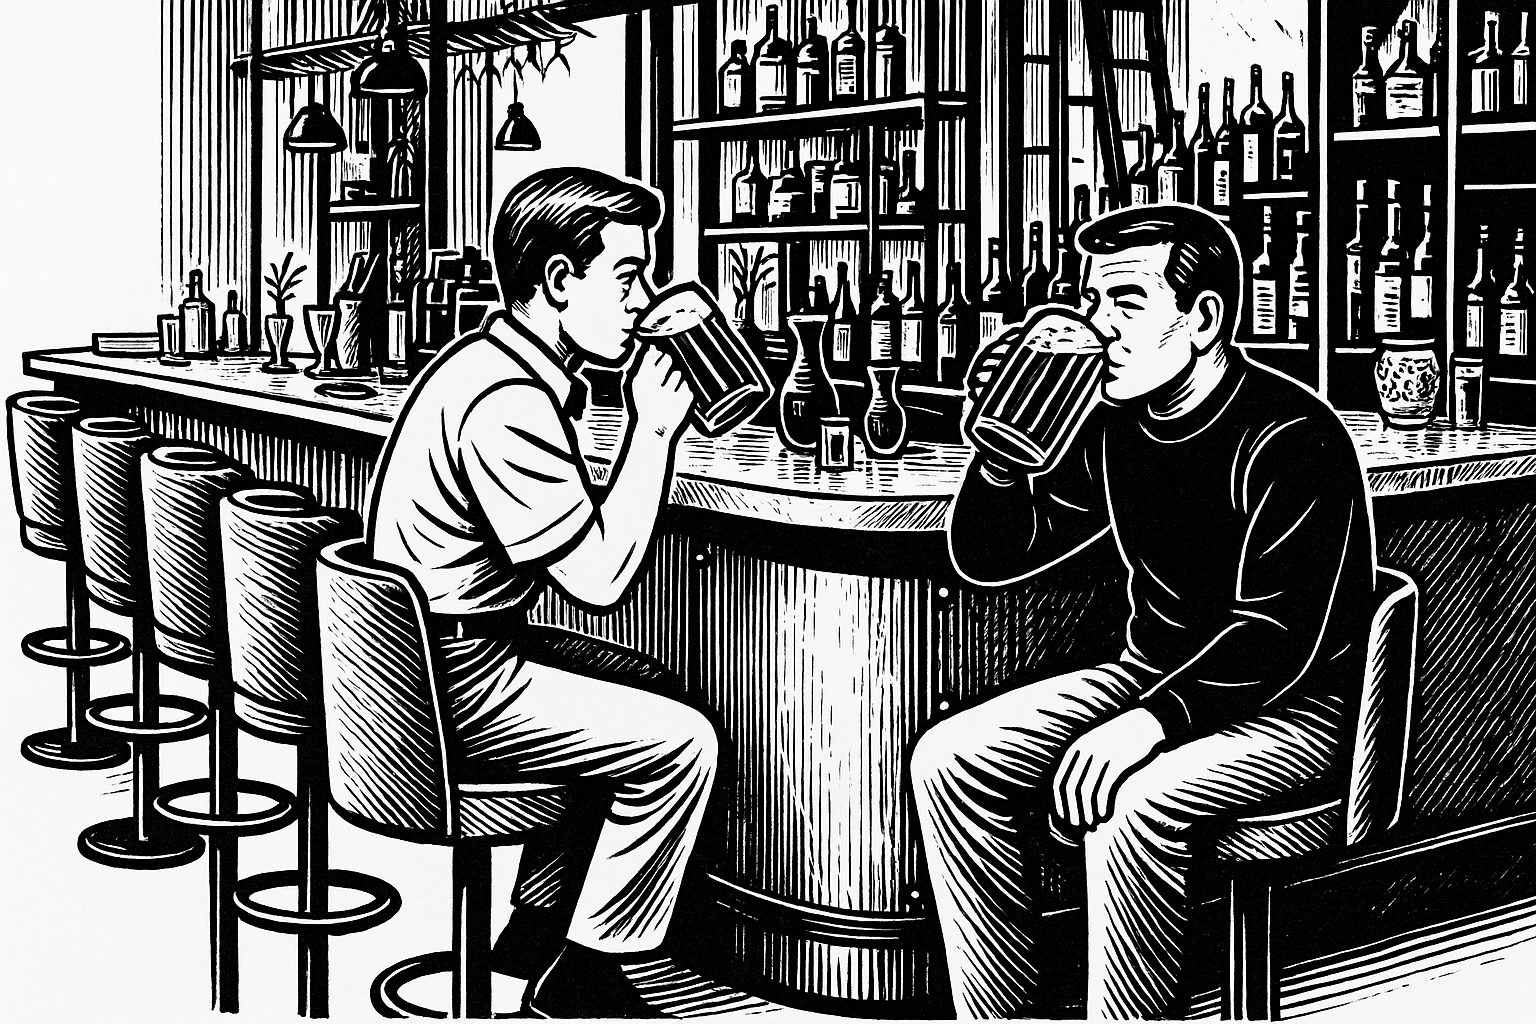
\includegraphics[width=1.0\textwidth]{3_new3}
	\caption{\small\textit{...Адмирал с Замполитом сидели в пивнушке...}}
	\end{figure}
	%\end{wrapfigure}

\diagdash Да\sdash a\sdash a, ну и маршрут ты выбрал$\ldots$\mdash Киря прихлебнул пенного и задумался.

\diagdash Не, ну или по старой схеме\mdash гоним в Чагоду и идём на Песь или Лидь.\mdash мгновенно сдал назад Шурик.

\diagdash Скукота, были уже.

\diagdash То\sdash то же. Итак, активная, с порогами, основная часть маршрута лежит по реке Суна. Это самая длинная река Карелии. Маршрут этот привлекает ещё и тем, что начало его относительно непопулярно. Карелия всё же намного более многолюдна в плане сплавщиков, чем чагодощенский край, так полюбившийся нам. А вот на <<Cунской цепочке>> народу поменьше, чем на других маршрутах, я прошерстил отчёты.\mdash вещал Шурик как лекцию.\mdash Плюс несложные пороги 2\sdash й категории. Посёлок Гирвас станет для нас базой заброски и выброски.\mdash закончил он и жадно прихлебнул из~кружки тёмного.

\diagdash Да\sdash a\sdash a, слушай, а на Кереть не думал?

\diagdash Думал, ты говорил уже. Я глянул, там в конце по~губе Чупа хреначить как\sdash то не круто. Да и севернее это всё намного. И~там пороги уже 3\sdash й категории есть, Кирь. Мы~командой ещё вторую не брали ни разу, не надо замахиваться на третью, тем более Серёга хреново плавает. 

\renewcommand*{\thefootnote}{\arabic{footnote}}
%\renewcommand*{\thefootnote}{\fnsymbol{footnote}}
\diagdash Кстати об этом$\ldots$\mdash Киря, взяв очередную кружку у бармена, отломил корюшки.\mdash Шурик, ещё раз, это КАРЕЛИЯ. Нам будут нужны спасжилеты, фартуки\footnote{Средство, защищающее гребца и байдарку от брызг, осадков, волн, а~также предотвращающее заливание байдарки водой в порогах.} на~байды, юбки\footnote{Приспособление в виде цилиндра из ткани, герметизирующее гребца, сидящего в фартуке, от волн и брызг.} на фартук.

\diagdash Кирь, это 2\sdash я категория, не 5\sdash я.

\diagdash Она будет для вас, салабонов, как 5\sdash я.

\diagdash Не гони, сам типа на опыте такой.\mdash огрызнулся Шурик.\mdash Был там раза три и рассказывает!

\diagdash Увидишь! Я ходил на Кереть, а остальные\mdash нет.

Шурик вдруг несколько осёкся, подумав, а что если Киря прав и они, как зелёные чайники, вляпаются в то, что им не по зубам? В конце концов, они все хотели некого баланса между отдыхом на полном расслабоне и экстримом порогов, а может получиться совсем не так. 

\diagdash Ладно, на днях поеду за снарягой. Ты прав, надо доукомплектовать байды.\mdash подытожил Шурик, и друзья, качаясь, вышли в вечернюю прохладу$\ldots$

%\vspace{0.9cm}
\vspace{0.5cm}
$\ldots$По команде в этот раз выходило трое точно и~Паша, а Юрич сказал, что на пороги точно не~пойдёт\mdash возраст, хоть Шурик и убеждал его в обратном, плюс заброска дальняя очень. Что ж, ударом это для товарищей не стало\mdash в~прошлом походе Юрич с трудом поднимался на высокие обрывы берегов, а с тех пор прошло ещё три года.

С Пашкой Шурик пересёкся на работе, обсудили как~и~что:

\diagdash Бензопилу берём! Вещь!!!\mdash глаза Пашки горели.

\diagdash Ку-ку?

\diagdash А чего? Нафига твои консервы там, компоты? Рыбы так наловим, халява!!! Зато дрова пилить бензой\mdash 30 секунд!

\diagdash Мда-а-а$\ldots$

\diagdash Ну как хочешь. Едем как?

\diagdash На машинах я и Серёга. Серёга повезёт кирину байду, мы\mdash мою, понятно. Ты и Киря\mdash со мной на тачке, а Серёга нашёл вроде ещё одного матроса на работе.

\diagdash Так, Сань, а рассадка?

\diagdash Короче, ты у~меня носовым гребцом и возражения не~принимаются\mdash мы идём на пороги и мне нужен опытный гребец спереди. Руслан, наш пятый, пойдёт вторым гребцом на нашей байде. Ну~а~вторая байда\mdash Киря как всегда кэп, а Серёга матрос на носу.\mdash изложил Шурик расклад.

\diagdash Ясно! Детали заброски?

\diagdash Через Старую Ладогу. Давай крепость посмотрим там древнюю?

\diagdash Хорошо, на том и порешили. Удочки я соберу, короче как обычно?

\diagdash Ну да$\ldots$

\diagdash Слушай, а там пороги что ли, да? Маршрут\sdash то покажи примерно?

\diagdash Пойдём на 2-ю категорию, пороги есть, во второй половине пути. Маршрут называется <<Сунская цепочка>>\mdash Шурик открыл карту.

\diagdash Ну в целом понятно.\mdash Паша быстренько окинул взглядом маршрут.\mdash Тебя подстраховать за рулём? Может без остановок тогда, раз два водителя?

\diagdash Не, нафиг. Устанем как черти. Да и крепость в~Старой Ладоге охота глянуть. Ты был там?

\diagdash Не-а.

\diagdash Вот никто из нас не был. Так что давай заброску разделим на две части\mdash c ночёвкой как раз в Старой Ладоге. Отдохнём с дороги, потом на следующий день осмотрим крепость и всё остальное как следует.

\diagdash Лад\'{ы}. Так, чё по снаряге? Раз пойдём пороги, спасжилет нужен, я так понял? И~неопренки? Ну, носки неопреновые? Или гидрокостюм? Ты~чё взял себе?$\ldots$

\diagdash Заказал гидроноски, будут на этой неделе. На верх\mdash термобельё на всякий случай, оно сохнет быстро. Спасы возьмём в~байдарочном магазе, вроде они норм там,\mdash показал Шурик сайт,\mdash что думаешь?

\diagdash Дорого! Я сам себе закажу чё попроще$\ldots$

\vspace{0.5cm}
$\ldots$Шурику позвонил Замполит:

\diagdash Выкладывай, Кирь.

\diagdash Всё пропало, Шурик, я никуда ни иду$\ldots$

\diagdash Ты охренел? Старт через неделю!!! Что стряслось, Штирлиц?\mdash Шурик вскипел буквально за секунды. Уж~кто\sdash кто, а Киря подвести не мог, просто не~имел права. 

\setcounter{footnote}{0}
%\renewcommand*{\thefootnote}{\arabic{footnote}}
\renewcommand*{\thefootnote}{\fnsymbol{footnote}}
\diagdash Да сходил сделал КТ\footnote{Компьютерная томография лёгких.} и у меня что\sdash то типа затемнения в лёгких, пульмонолог ещё насел с моим курением и всё такое$\ldots$

\diagdash Фух! Я\sdash то думал!!!\mdash у Шурика немного отлегло.\mdash Это они тебя стращают, чтоб ты курить бросил, ёпрст! Завязывай, Кирь. Конечно затенение, смолишь как паровоз! Кончай шуточки, пакуй гермы! На тебе пахать можно!

\diagdash Думаешь?

\diagdash А то! Если до тебя к этому врачу ещё ходила твоя жена, то эт ваще как в анекдоте: <<Больной, вам нельзя пить, курить, играть в карты и увлекаться случайным сексом!>>

\diagdash Хар\'{о}ш, я ведь серьёзно$\ldots$

\diagdash Я тоже! После ковида не восстановился может, туда\sdash сюда! Не вздумай слиться, трибунал не оценит! На кой только чёрт ты попёрся на КТ?!$\ldots$\mdash Шурик негодовал, но вроде ему удалось внушить Кире, что опасения явно преувеличены. Тот согласился. Согласился, в конце концов, и консилиум врачей. Замполит был спасён. А Шурик в~очередной раз подумал, что как его уже задолбало всех собирать, сплачивать в команду\mdash хоть разочек бы кто всё это организовал: продумал маршрут, договорился о~заброске, собрал снарягу, закупил провизию, а он бы просто соизволил приехать поучаствовать$\ldots$

%\newpage
%\vspace{1.3cm}
\vspace{0.5cm}
%\renewcommand*{\thefootnote}{\arabic{footnote}}
\renewcommand*{\thefootnote}{\fnsymbol{footnote}}
$\ldots$Поскольку <<Сунская цепочка>>\mdash всё таки 2\sdash я~категория, ребята решили прикупить спасжилеты, спасконец Александрова\footnote[1]{Средство для оказания помощи утопающим\mdash представляет собой плавучий тонкий трос, длиной около 30\thinspace м; кидается утопающему в~специальном мешочке, обеспечивающем точность броска и последующее разматывание троса в полёте.}, фартуки для байдарок и~байдарочные юбки. Словом, подготовиться к бурной реке. Опыт сплава по~категорийной реке был только у~Кири\mdash он ходил и~по~Шуе, и~по~Керети в Карелии, но$\ldots$ в детстве. Сейчас же у Кири и Шурика были собственные корабли и~предстояло дооснастить их для плавания по~порогам. 

В пятницу после работы Шурик в~гордом одиночестве поехал покупать байдарочную снарягу. Сойдя с электрички, он набрал давно осевший в~телефонной книге номер:

\diagdash Да?\mdash внезапно ответил молодой, но томный женский голос.%, хотя контакт был на мужика.

\diagdash Я насчёт снаряжения, общались по электронке$\ldots$\mdash и они договорились встретиться на углу улицы, поскольку прежний ориентир\mdash старые гаражи, где у этих деятелей была мастерская по изготовлению байдарочных оболочек и~снаряги\mdash снесли.

\diagdash Как я вас узнаю?\mdash спросил Шурик.

\diagdash Узнаете, поверьте!


\begingroup
\justifying
\parfillskip=0pt % <- это заставит последнюю строку растягиваться
	
Через пару минут он увидел невысокую черноволосую девушку с~хитрым~прищуром, которая~тащила~ярко\sdash оранжевые~спасжилеты~и~два 

\par
\endgroup

\noindent
\begin{minipage}{0.55\textwidth}
	\setlength{\parindent}{1.0cm}  % Включаем красную строку
	\setlength{\parskip}{0.25cm}     % Межабзацный отступ, как в основном тексте
	
	\noindent байдарочных фартука, надев их на себя. Узнал издалека, не~ошиблась.
	
	\diagdash Так, вот, держите,\mdash стала передавать, снимая с~себя снарягу, байдарочница, а~Шурик стал навешивать фартуки и~жилеты уже на~себя.
	
	\diagdash А остальное?	
	
	\diagdash А остальное на другом складе, надо пройти минут пять, пошли?\mdash маняще мотнула она головой в~сторону 9\sdash этажек и поправила волосы$\ldots$
\end{minipage}\hfill
\begin{minipage}{0.40\textwidth}
	\centering
	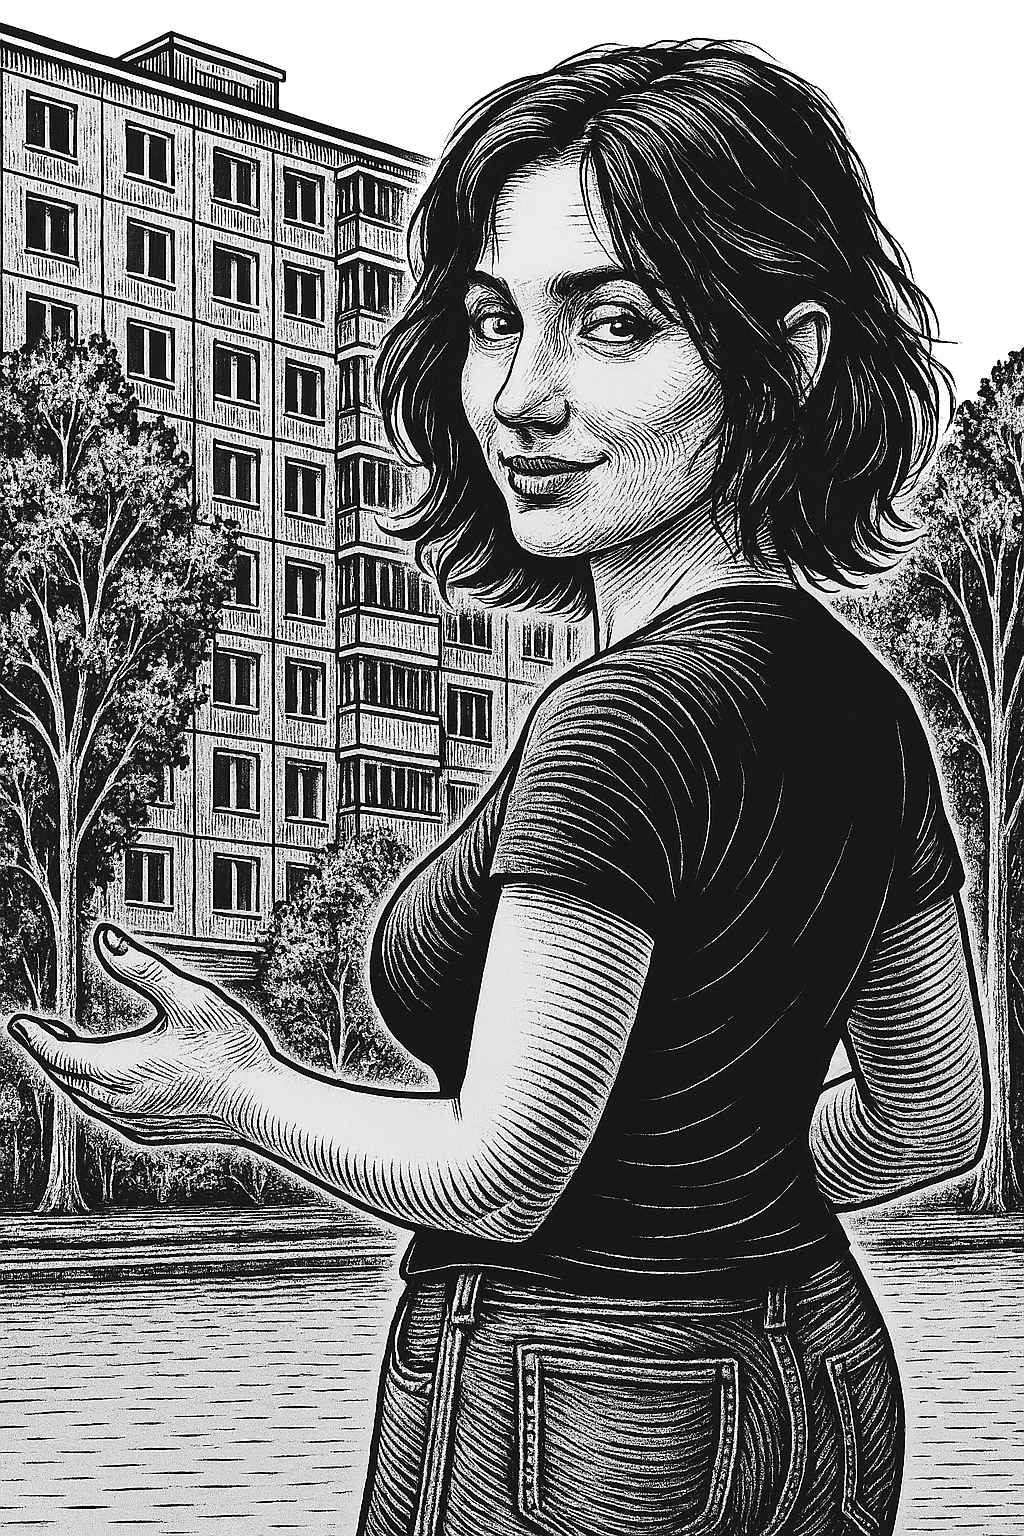
\includegraphics[width=\linewidth]{3_1_new2}
	
	{\small\textit{...с~хитрым~прищуром...}}
\end{minipage}

%Через пару минут он увидел невысокую черноволосую девушку с хитрым прищуром, которая тащила ярко\sdash оранжевые спасжилеты и~два байдарочных фартука, надев их на себя. Узнал издалека, не~ошиблась.

%\vspace{1.0cm}
\vspace{0.5cm}
%$\ldots$Спустя полчаса 
$\ldots$Шурик, весь увешанный снарягой в~количестве двух огромных фартуков на~байдарку\sdash двушку и трёшку, пяти юбок по количеству людей в команде, двух заглушек грузовых отсеков, двух безнадувных ярко\sdash оранжевых спасжилетов и остального по~мелочи, дождался такси. Усевшись на пассажирское, он~набрал Кире:

\diagdash Мне тут такая снарягу только что продала$\ldots$ Фартуки, юбки и все дела. Жди,~скоро буду у тебя, барахла полный багажник.

\diagdash Хах, ты аккуратнее там со случайными связями.\mdash не преминул ввернуть тот. %А~пивка, лад\'{ы} уж, оставим тебе, так и быть!

Через час ребята затащили домой к Кире снарягу и~собрались уже в <<пивотеку>> на 1 этаж, как вдруг Шурик вспомнил про топокарты:

\diagdash Кирь, ты говорил, что у тебя ламинатор есть?

\diagdash Ага, есть у нас.\mdash Надя, кирина жена, вдруг появилась в квартире как будто из ниоткуда.

\renewcommand*{\thefootnote}{\fnsymbol{footnote}}
\diagdash О! Отлично! Заламинируем карту похода?\mdash Шурик вчера в очередной раз просидел до двух ночи над~лоциями, описаниями маршрута, нанося на~распечатанные карты свои условные обозначения\mdash районы стоянок он помечал флажками по офицерской линейке, мосты, под~которыми надо будет проплывать, обводил кружками, названия порогов\mdash подчёркивал. Такая <<поднятая>>\footnote[1]{Поднять карту\mdash выделить на ней что\sdash либо цветом и/или дополнительными условными обозначениями.} карта смотрелась уже намного читабельнее. Плюсом, пока Шурик проделал всё это, он уже почти запомнил маршрут, местность, ключевые ориентиры.

\diagdash Ничего себе! Это вы всё пройдёте?!\mdash Надя была явно в тихом шоке от маршрута.\mdash Это же пороги?!

\diagdash Ну да, пороги$\ldots$ Блин, перегрели!!! Повело плёнку!\mdash Шурик в панике вытаскивал из ламинатора первый лист.% карты похода.

\diagdash А дубликат есть?\mdash заволновалась Надя.

\diagdash Нет уж, пойдём по такой карте.\mdash Замполит деланно закатил глаза.\mdash Потеряемся, как пить дать! Ё\sdash моё! Ну всё, Шурик, по такой карте идти нельзя! 

\diagdash Всё пропало, Кирь!\mdash подыграл тот.

\diagdash Да вы чего?\mdash Надя посмотрела на них обоих.

\diagdash Забей, я весь маршрут уже наизусть помню, погнали скорее в <<Пивотеку>>\mdash хорохорился Шурик.\mdash Доделываем, пиво греется, ё-моё!$\ldots$

\vspace{0.5cm}
$\ldots$Спустя пару часов пивотекошная братия во главе с~Кирей сажала Шурика в такси вместе с его частью снаряги. Он опирался на чьи\sdash то плечи справа и слева, расставив руки как на картине Константина~Васильева <<Илья Муромец и~голь кабацкая>>. Через ещё минут 40 он, пошатываясь, открыл своё авто, припаркованное прямо перед подъездом, и~с~трудом затрамбовал купленные спасжилеты и остальную снарягу в и без того уже набитый походным барахлом багажник, погладил байдарку в~упаковке и побрёл домой. Вокруг стояла тёплая июльская ночь. Дома, не спя, ждала~жена$\ldots$

\begin{center}
	\psvectorian[scale=0.4]{88} % Красивый вензелёк :)
\end{center}
